\documentclass{beamer}
\usepackage[utf8]{inputenc}
\usepackage{listings}
\usepackage{multicol}
\usepackage{graphicx}


\usetheme{Frankfurt}
\usecolortheme{default}


\title[Crisis]{Introduction to contract programming}
\author{Łukasz Ziobroń}
\institute{Nokia}
\date{Code Dive Community, 2015}
\subject{Computer Science}
\lstset
{
    language=C++,
    numbers=left,
    basicstyle=\ttfamily\scriptsize,
    keywordstyle=\color{blue}\ttfamily,
    stringstyle=\color{red}\ttfamily,
    commentstyle=\color{green}\ttfamily,
}
\graphicspath{ {./img/} }
\DeclareGraphicsExtensions{.pdf,.png,.jpg}


\begin{document}


\begin{frame}
\titlepage
\end{frame}

\begin{frame}
\frametitle{Table of Contents}
\begin{multicols}{2}
\tableofcontents
\end{multicols}
\end{frame}

\section{Some examples}
\subsection{Ariane 5 mission}
\begin{frame}
\frametitle{Ariane 5 mission}
\only<1>{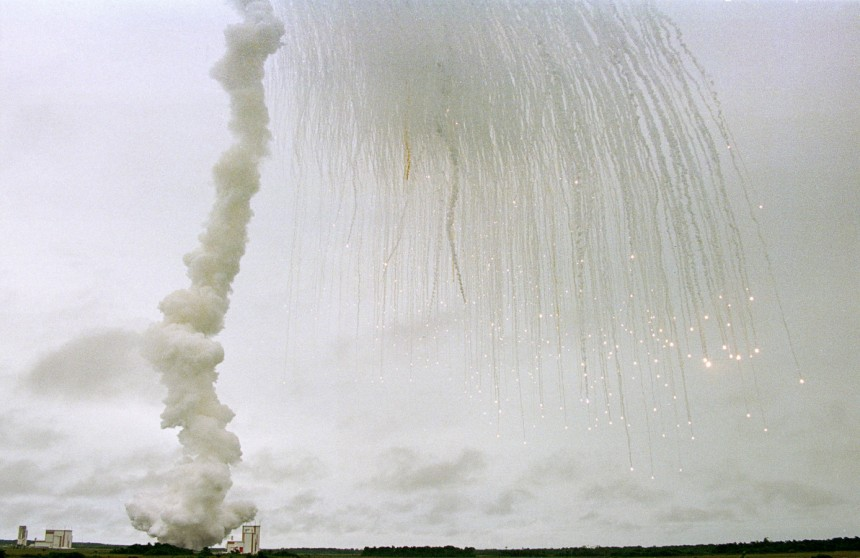
\includegraphics[scale=0.35]{ariane}}
\only<2>
{
  In 1996, the Ariane 5 rocket was reusing software from the Ariane 4. 37 seconds after its maiden launch the self-destruct safety mechanism was activated. \\~\\
  A data conversion from 64-bit floating point value to 16-bit signed integer value to be stored in a variable representing horizontal bias caused a processor trap because the floating point value was too large to be represented by a 16-bit signed integer. \footnote{https://en.wikipedia.org/wiki/Ariane\_5\#Notable\_launches} \\~\\
  This bug, existing in Ariane 4 software never came out on Ariane 4 rocket.
}
\end{frame}

\subsection{Calculator source code}
\begin{frame}[fragile]
\frametitle{Basic calculator}
\only<1>{ \lstinputlisting[linerange={13-23}]{"src/calculator.cpp"} }
\only<2>{ \lstinputlisting[linerange={25-40}]{"src/calculator.cpp"} }
\end{frame}

\subsection{code with checks}
\subsection{additional validation}
\subsection{how much we added?}
\subsection{can we do better?}

\section{Let's define contract}
\subsection{what is a contract?}
\begin{frame}
\frametitle{Contract by Design}
\framesubtitle{What is it?}
Contract defines our rights and responsibilities and rights and responsibilities of the other side as well.
Design by Contract (DBC) is a programming technique invented by Bertrand Meyer.
It assures that every function implementes a particular behaviour and requires 3 things:
\end{frame}

\begin{frame}
\frametitle{Contract by Design}
\framesubtitle{3 expectations}
\only<1-3>{
\begin{block}{Preconditions}
Required to call the function. Function should never be called if its preconditions are not satisfied.
\end{block}}

\only<2-3>{
\begin{block}{Postconditions}
Describes the state of the world after the function call.
\end{block}}

\only<3>{
\begin{block}{Class Invariants}
The class guarantees that invariant is always true between function calls. It means that during function call invariant may not be satisfied, but after function execution it must be satisfied.
\end{block}}

\end{frame}


\subsection{what is our contract}
\subsection{source code with contract}
\section{How does it work?}
\subsection{Preparsing}
\subsection{Code generation}
\subsection{example of generated code}
\section{Different languages}
\subsection{C++ - nana}
\subsection{Java - iContract}
\subsection{D - built-in mechanism}
\subsection{Eiffel - it started here}
\subsection{C++ - assertions}
\section{Some statistics}
\subsection{Code bloat - numbers}
\subsection{C++ - without, validations, contracts, generated}
\subsection{Java}

\section{Summary}
\subsection{Q \& A}
\begin{frame}
\frametitle{Q \& A}
\begin{center}
\Huge Questions?

\includegraphics[scale=0.45]{dice_questions}
\end{center}
\end{frame}



\begin{frame}{Przyklad 2 kolumn}
Coś tam cośżźćł
\begin{columns}[t] % wyrownanie do gory
\column{.5\textwidth}
Tresc pierwszej kolumny
\column{.5\textwidth}
% \includegraphics[height=3cm]{rys.png}
cośisko
\end{columns}
\end{frame}

\begin{frame}
\begin{block}{To jest blok}
Jakas informacja
\end{block}

\begin{alertblock}{To jest Alert block}
Jakas wazna informacja
\end{alertblock}

\begin{exampleblock}{To jest Example block}
Jakis przyklad
\end{exampleblock}
\end{frame}


\end{document}
